\documentclass{standalone}
\usepackage{tikz}
\usepackage{schemabloc}

\begin{document}

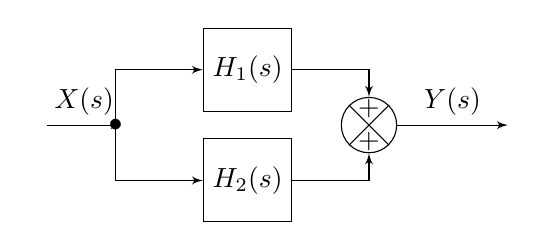
\begin{tikzpicture}
  % Entrée
  \sbEntree{E}
  \sbCompSum[12]{C1}{E}{+}{+}{}{}
  \node [right of=E] (n1){$\bullet$};
  \node [right of=E, node distance=1.2cm] (n2){};
  \sbRelier[$X(s)$]{E}{n2}

  % Premier bloc en haut
  \sbDecaleNoeudy[2]{E}{A1}
  \sbBloc[6]{B1}{$H_2(s)$}{A1}
  \sbRelieryx{n1}{B1}

  % Deuxième bloc en bas
  \sbDecaleNoeudy[-2]{E}{A2}
  \sbBloc[6]{B2}{$H_1(s)$}{A2}
  \sbRelieryx{n1}{B2}

  % Somme
  \sbRelierxy{B1}{C1}
  \sbRelierxy{B2}{C1}

  % Sortie
  \sbSortie[4]{S}{C1}
  \sbRelier[$Y(s)$]{C1}{S}
\end{tikzpicture}

\end{document}
